\documentclass{article}
\usepackage[utf8]{inputenc}
\usepackage{pdfpages}
\usepackage{minted}
\usepackage{hyperref}
\usepackage{enumitem}
\usepackage{graphicx}
\usepackage[margin=1in]{geometry}
\graphicspath{ {images/} }
\title{RBE/CS549 Project: Boat Tracking/Detection}
\author{Jordan Burklund \and James Kuszmaul}
\begin{document}
\maketitle

\section{Task}

We are currently working on a robotic sailboat for the
International Robotic Sailing Competition (\url{http://sailbot.org}).

In navigating a sailboat, we would like to be able to
detect and maneuver around various objects
that are floating on the surface of the water. As such,
it is desirable to be able to (a) identify and (b)
predict the motion of objects on the water. Computer
Vision is a potentially convenient way to do this.
We are not specifically aware of any particularly
thorough published work on this particular application
(while we have used vision in the past, it has been
extremely simple detection of bright-colored buoys
on the water).

The goal of this project shall be to use some existing
video to try and detect and track objects in video,
and to understand how well we can develop such a
detector without having a labelled dataset. We will,
for the time being, not worry about being able to run
the algorithm in real time onboard the boat (although
practical considerations mean it must be able to
perform fast enough for us to evaluate it).

\section{Data}

We have approximately 240GB of HD video from a GoPro
mounted on the prow of a large motorboat. While we
do not have the processing power to fully take advantage
of every frame of data, we will pull reasonable samples
of data to work with.  Specifically, we will generate a test dataset of reduced sized that includes the following important characteristics:

\begin{itemize}
\item With/without land (to see different horizon conditions).
\item Varying amounts of other objects/traffic.
\item Areas with significant camera movement in either pitch or roll (may extend to both pitch and roll depending on progress).
\item Different water conditions (starting with flat, calm water, and progressing to more chaotic water conditions as time allows)
\item Objects both near/far away (including near the horizon)
\item Frames that include water droplets on the lens
\end{itemize}

The boat that the data is collected on is relatively stable
and the GoPro is mounted in the same spot for the length
of the video. As such, we should be able to safely ignore
the rotational pose of the boat (when we apply these
algorithms to our final boat, we will have to account for
the much more noticeable movement of that boat).

\begin{figure}[H]
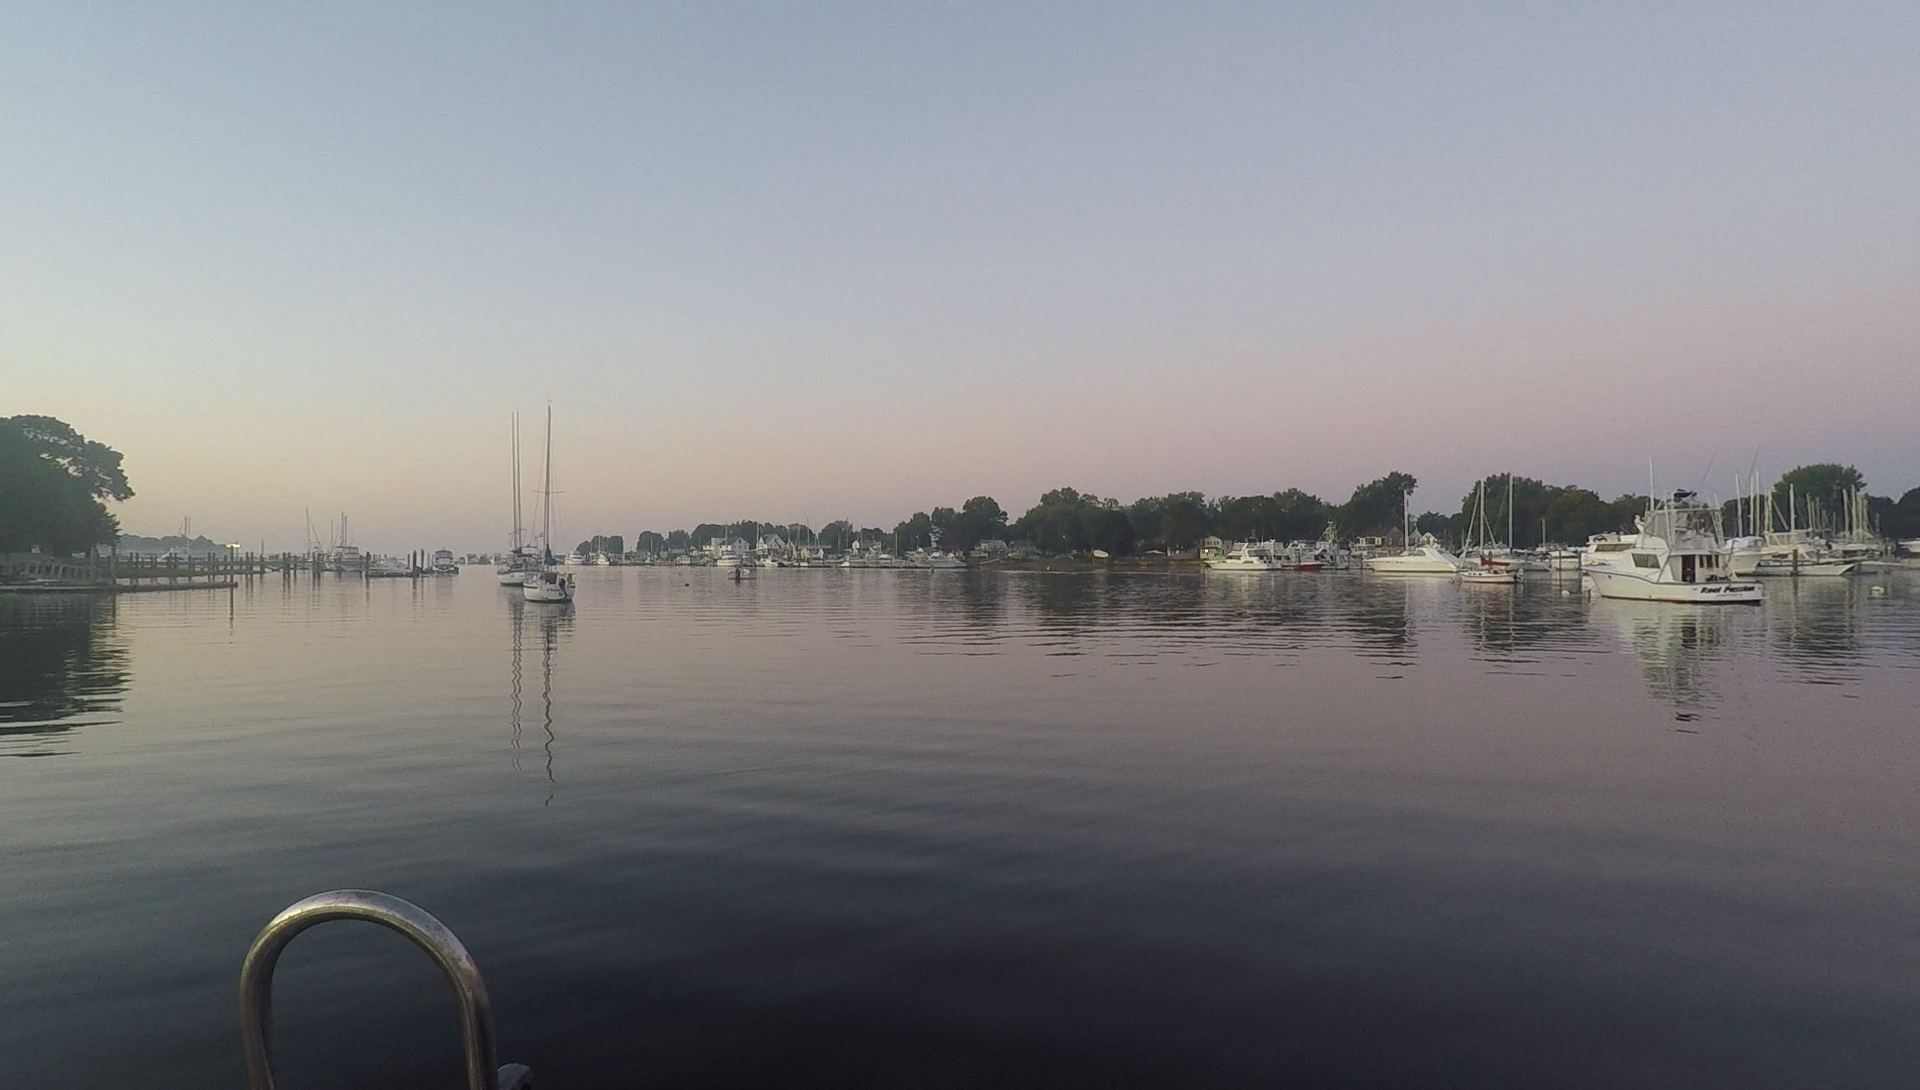
\includegraphics[width=12cm]{sample1}
\centering
\caption{Sample image 1}
\end{figure}
\begin{figure}[H]
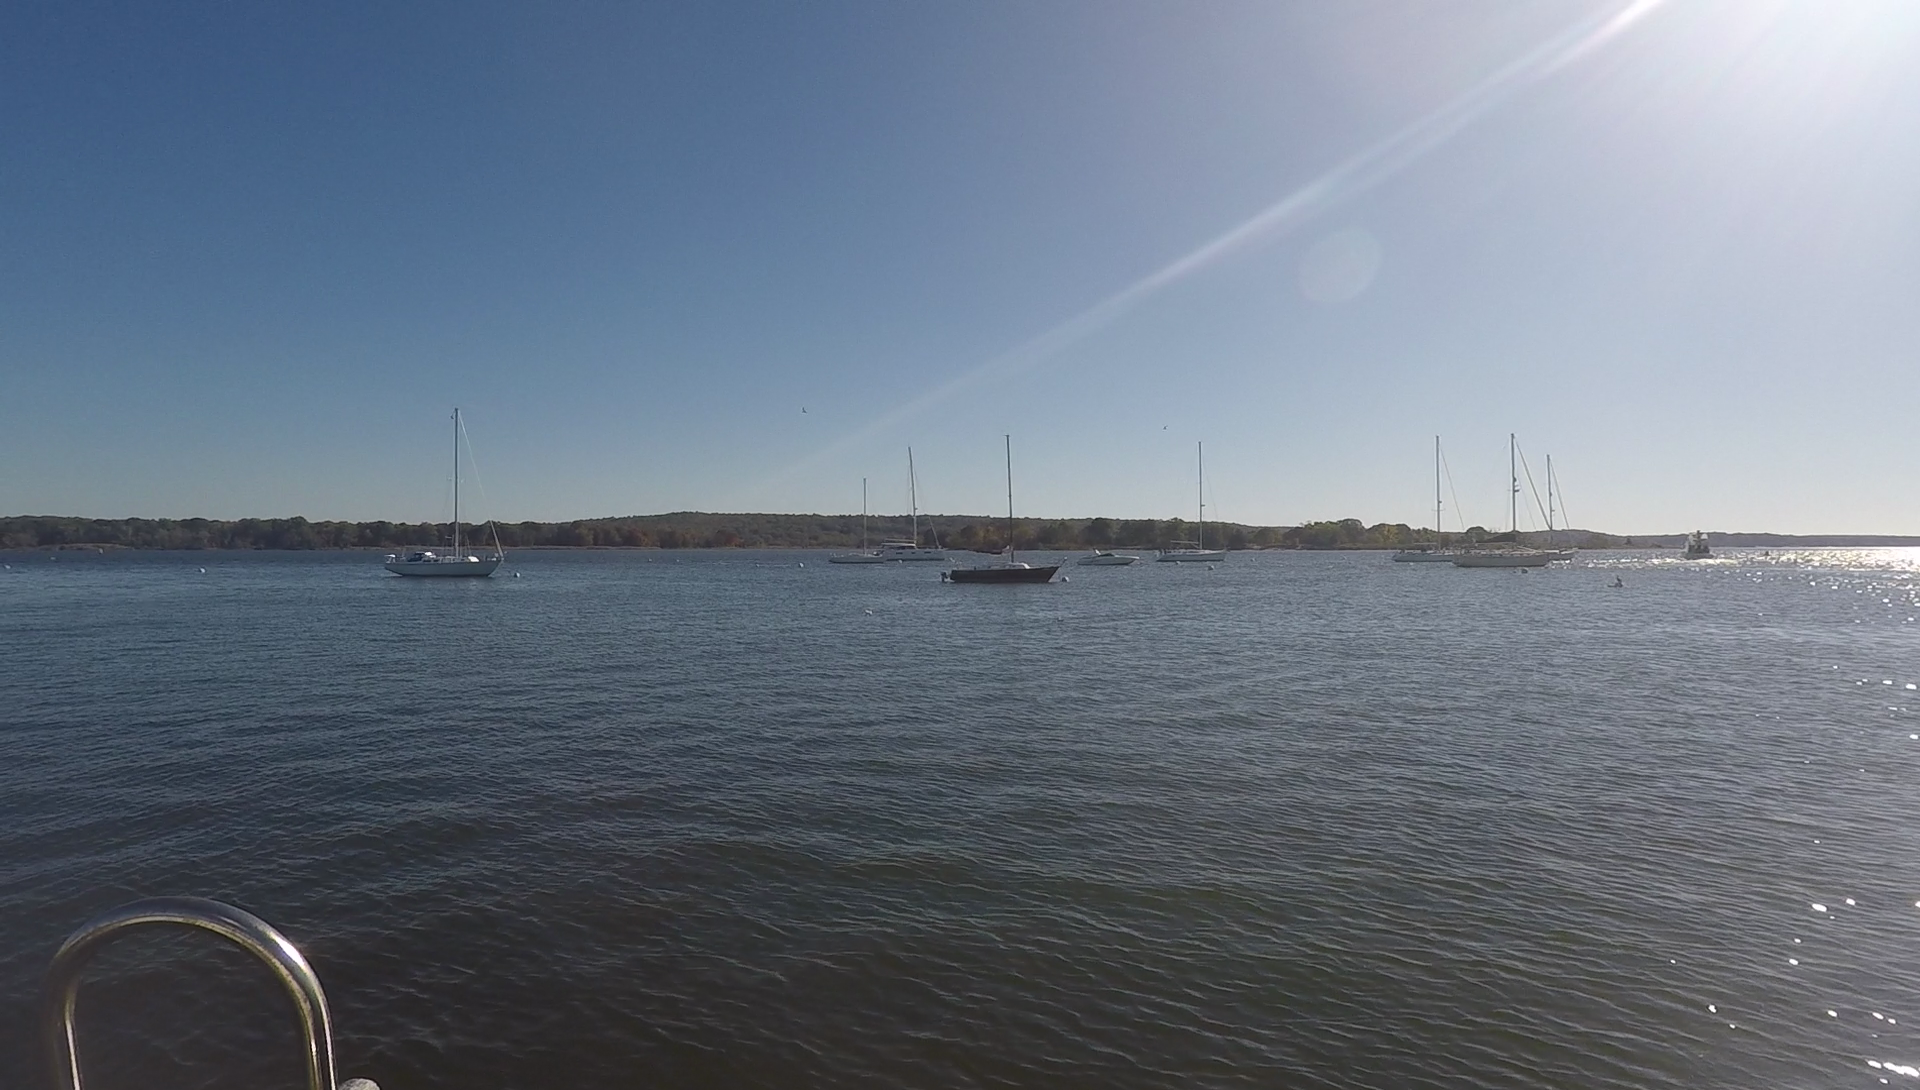
\includegraphics[width=12cm]{sample2}
\centering
\caption{Sample image 1}
\end{figure}


\section{General Approach}

Overall, the object pipeline is as follows:

\begin{enumerate}
\item We read a frame of video and convert it to HSV space
\item Perform a slew of static transforms to try and determine,
      based on the content of a single frame, which areas are and
      are not water/sky/land/objects
\item Use optical flow information from a given pair of frames to
      locate the moving objects in a frame
\item Combine the above to determine a set of viable blobs
\item Associate the blobs with each other and with preexisting objects,
      creating new objects for blobs that can't be associated with any
      preexisting objects
\item Update objects in preparation for the next frame, updating
      positions using velocities, reducing and increasing confidence
      scores as appropriate, deleting objects with sufficiently low
      scores
\end{enumerate}

\section{Image Segmentation}

\section{Optical Flow}

For the underlying optical flow algorithm, we use Farneback's
[INSERT CITATION HERE] which is accessible in matlab as...

\section{Evaluation Section from Proposal}

Because we do not have a labeled data set, we must develop
some way evaluate the performance of different algorithms.

In order to do this, we propose two general cost functions.
The first will evaluate the motion tracking features.
Essentially, when motion tracking, our objective is to
correctly predict the future path of an object. As such,
the cost function will assume a sane object detector and
use the difference between predicted frame-to-frame position
and actual frame-to-frame position (from the object detector)
as the cost.

For the object detector itself, a bit more complication is
required, and we hypothesize that the cost function will
consist of the following terms:

\begin{description}
\item[Object Deletion] Any unexpected object deletion shall
   be penalized, in order to avoid constantly losing track
   of objects between frames or over/under segmentation of
   individual objects. ``Expected'' object deletion would
   occur when an object that is already moving out of frame
   or behind another object disappears. In theory we also
   care about excessive object \emph{creation}; however,
   because the vast majority of created objects are also
   deleted eventually, the additional complication should
   be unnecessary. There is an open question about how
   to treat the deletion of objects that disappear over
   the horizon; however, such occurrences are hopefully
   rare enough or easily detectable enough that their
   cost should be insignificant (we don't want to
   accidentally \emph{not} penalize flickering objects
   that happen to fall on the horizon).
\item[Number of Objects] In order to avoid either a
   detector that never deletes objects or one that
   divides real objects into far too many individual
   objects, we shall penalize the number of objects
   identified in any given frame. This may be quadratic
   or some higher order function in order to avoid
   penalizing small numbers of objects excessively.
\item[Unaccounted for Area] To avoid an object
   detector that simply never returns any objects,
   we shall compare the area accounted for by the
   identified objects and the area that ``should''
   contain objects (per some naive estimate), and
   penalize any unaccounted for area.
   As an initial method for identifying this area,
   we propose that we (a) develop some simple detector
   for identifying sea water (it's mostly blue...),
   and (b) make a simple assumption about the location
   of the horizon (the existing video is relatively stable,
   so the horizon should be, and this way we won't have
   to worry about the sky). Any area below the estimated
   horizon that is not sea water ``should'' be part of
   an object (this includes the shore).
\end{description}

Obviously, the above cost function will not provide a perfect
measure of algorithm performance. However, between it and
qualitative sanity checks, we should be able to provide
a good estimate of the performance of our algorithms.

\section{Responsibilities Section from Proposal}
\begin{description}
\item[James Kuszmaul] Work on basic object detection and how
  to retain object associations between frames/measure .

\item[Jordan Burklund] Develop methods to segment and mask pixels that represent water. Explore methods using contours for object detection.
\end{description}
\end{document}
